\section{Route Instructions}

\subsection{Types of Route Instructions}
There are three types of route instructions:

\begin{itemize}

\item Numbered -- Complete the Numbered Route Instructions (NRIs) in ascending numerical order.  An NRI is active (available to be initiated) when all parts of the preceding NRI have been completed.  Initiate (begin) an NRI when you reach its first reference point.

\item Note -- Notes are unnumbered route instructions.  A note is active from its introduction until cancelled.  A note may be executed once, more than once, or never.  Action must be taken as directed each time the appropriate action point is encountered.  Notes supersede but do not cancel NRIs.  Notes are independent of and may overlap NRIs.  Canceling a note does not cancel its associated speed.

\item Supplemental -- Supplemental route instructions are usually provided at checkpoints and route controls.  Complete all the supplemental route instructions in the order presented (usually alphanumerically) before resuming the NRIs.

\end{itemize}

When a route instruction consists of multiple actions, each action is to be executed in the order given, at the first opportunity.  A route instruction is complete when all parts of the instruction have been completed.  Route instructions can refer to other route instructions, reference points, or action points.

\subsection{Action Points}
An action point is the location where a route instruction is executed.  An action point can be any of the following:

\begin{itemize}

\item An intersection where the route instruction directs you off the main road.

\item An intersection where a route instruction with official mileage directs you to follow the main road.

\item An intersection where a route instruction labeled MBCU directs you to follow the main road.

\item The indicated point, distance, or duration where no change of direction is specified in the route instruction.

\end{itemize}

\subsection{Reference Points}
A reference point is accompanied by an official mileage, has an identifying sign, or is defined in the glossary of these Road Rally Rules or the glossary of the event's supplemental rules.  A reference point marking the beginning of a route instruction will occur at a mileage greater than the mileage of the action point marking the end of the previous route instruction.  Route instructions labeled API may reference the action point of a previous instruction.

\subsection{Landmarks}
A Landmark is a physical object identified by a sign.  A landmark is identified in route instructions in upper case (all capital letters) not in quotation marks (``'') and is not a term defined in the Glossary.

\subsection{Deviations}
A deviation is a change in course off the main road. L, LEFT, R, RIGHT, S, STRAIGHT, and TURN are deviations.  Route instructions may contain more than one deviation.

\subsection{Official Mileage (OM)}
Route instructions that are accompanied by OM must be executed at that mileage provided that:

\begin{itemize}

\item The reference is correct and

\item An appropriate action point exists

\end{itemize}

Deviations referenced by an OM may be executed to follow the main road.  Contestants will not be required to determine OM to greater precision than 0.1 (one-tenth) mile in order to determine the rally route.

\subsection{Alpines}
An alpine is a diagram drawn to represent an intersection or group of intersections as closely as possible.  The dot in the alpine represents the road on which the contestant enters the intersection(s) and an arrowhead indicates the road on which the contestant leaves.  If more than one legal route exists, take the shortest legal route through the intersection(s).  A speed change associated with an alpine instruction is executed as you enter the first intersection in the diagram.  Alpines are not subject to the MRDs (see Section \ref{sec:mrd} on page \pageref{sec:mrd}).

\begin{quote}
EXAMPLE:
\begin{picture}(0,0)
 \setlength{\unitlength}{1pt}
 \put(0,0){\tiny NRI 23.}
 \put(20,-15){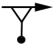
\includegraphics[width=.45in]{Example_Tulip_Diagram.png}}
 \put(40,-10){\tiny CAST 34}
\end{picture}
\end{quote}


\subsection{Speed Changes}
Speed changes that occur at an intersection are executed as you enter the intersection.  Speed changes that occur at a reference are executed as you pass by and are even with the reference.  When a speed change is to be done for a specified time or distance, you revert to the previous speed after the specified time or distance.

\subsection{Comments}
Text within parentheses (()) is to be considered clarifying comments.  Any action suggested within parentheses, while probably helpful, is not mandatory.

\begin{quote}
Example:\\
25. L at STOP. (Use caution, traffic does not stop.)
\end{quote}